% ---------------------------------------------------------------------
%  4  RESULTS AND DISCUSSION
%  Numbers from the last runs (data from 2020) of classical-models.ipynb,
%  neural-models.ipynb and timestral-zero-shot.ipynb
%  (test block, Jul 2024 -- Oct 2026).
% ---------------------------------------------------------------------
\section{Results and Discussion}
\label{sec:results}

Table~\ref{tab:main} summarises the test results; every model in it was
chosen without the test block.

\begin{table*}[t]
\centering
\caption{Test-block results (Jul 2024 -- Oct 2026) of the models chosen
on train and validation, against the best simple rule. Brackets: 95\%
block-bootstrap intervals.}
\label{tab:main}
\footnotesize
\setlength{\tabcolsep}{4pt}
\begin{tabular}{@{}L{3.0cm}L{3.6cm}L{5.9cm}L{3.1cm}c@{}}
\toprule
Question & Chosen model & Test result & Simple rule & Beats rule? \\
\midrule
24 hourly returns (assigned task) & tuned linear, KNN, trees, MLP, LSTM
  & MAE skill $-0.0004$ to $-0.0002$ (networks to $-0.0020$); IC
    $\le 0.021$; DM $p \ge 0.15$
  & zero forecast & no \\
Direction of the next hour & GB classifier (base + Binance)
  & AUC 0.538; 56.0\% right on top-10\% calls ($p=5\cdot10^{-8}$)
  & last-hour reversal: AUC 0.528 & yes, small \\
Size $|\ret|$ of each next hour & Timestral + GB refitted monthly
  & $\Rtwo = \mathbf{0.164}$ (Timestral 0.157, LSTM 0.156, GB 0.148)
  & last week $\times$ hour profile: 0.056 & yes \\
80\% range for each next hour & GB quantile + rolling Mondrian conformal
  & coverage 80.0\% (calm 78\%, wild 82\%, release hours 82\%), width
    0.98\%; Timestral uncalibrated: 80.3\%, 1.00\%
  & fixed range: 87.6\%, 1.28\% & yes \\
Next-day return & Ridge & $\Roos = -0.001$, IC 0.051 & zero forecast & no \\
Next-day direction & Random Forest & AUC 0.509, accuracy 49.9\%
  & always up: 50.1\% & no \\
Next-day volatility & top-3 tree ensemble; GB refitted monthly
  & $\Rtwo = 0.510$ [0.45, 0.56]; 0.517 & last week's mean: 0.094 & yes \\
Volatility targeting (economic) & next-day volatility forecast
  & Sharpe 0.27, max.\ drawdown 64\% & buy \& hold: 0.50, 53\% & no \\
\bottomrule
\end{tabular}
\end{table*}

\subsection{Hourly Returns: the Assigned Task}
\label{sec:res_returns}
No model forecasts the 24 hourly returns better than ``no change''. Every
tuned classical model ends within 0.0001 percentage points of the MAE of
the zero forecast (0.3193\%), the long-format models have $\Roos$ within
$\pm0.001$ of zero (Diebold--Mariano $p\ge0.15$), and the networks and
the median of Timestral do no better. More model freedom always meant
worse validation scores, and the chosen Ridge needs $\alpha=10^5$, i.e.\
it shrinks almost to zero: the signature of a target that is mostly
noise. Choosing models by the squared-error criterion they were trained for,
rather than by MAE, raises the IC from 0.003 to 0.021, with an interval
$[+0.006, +0.035]$ that excludes zero, but this ranking signal is too weak
for the forecast itself to beat zero. At the
hourly scale Bitcoin is close to a random walk, as Fig.~\ref{fig:acf}
suggested and as market efficiency predicts~\cite{fama1970}: a
predictable direction would be traded away.

\subsection{Next-Hour Direction}
\label{sec:res_direction}
The one exception is the next hour. The rule ``the next hour moves
against the last one'' reaches AUC 0.528 and is right 54.6\% of the time
on its 10\% most confident calls ($p=2\cdot10^{-5}$); GB with Binance
order-flow features adds a little (AUC 0.538, 56.0\%). An LSTM reaches
the same AUC only when trained on every origin, which helps GB as much
(0.541), so the data, not the network, makes the difference. The effect
is real but small, measured before trading costs, and vanishes from the
second hour on: hours 2--24 and the next day are a coin flip.

\subsection{Size of the Hourly Moves}
\label{sec:res_size}
The size of the moves is where the models have clear skill
(Fig.~\ref{fig:size}). The long format was the largest modelling gain
(validation $\Rtwo$ 0.052 to 0.097, same model and features). On test, GB
fitted once explains 13.1\% of the variance of each hourly $|\ret|$,
against 5.6\% for the volatility rule (gain $[+0.057, +0.084]$); its skill
falls from about 0.16 one hour ahead to 0.11 at 24 hours, as recent
volatility says less about later hours. Refitting every month raises
$\Rtwo$ to 0.148 ($+0.017$ $[+0.010, +0.024]$, better in 20 of 29
months): in a drifting market (Fig.~\ref{fig:hour}), keeping the model
current is worth more than any extra input. None of the candidate features
from the analysis, nor Binance and ETH, improved the trees ($-0.0004$
$[-0.004, +0.003]$ after refitting): recent volatility and the clock
already carry their information. Release hours stay under-predicted (0.65
times their actual size): with 544 training rows they are fewer than one
leaf of the tuned GB, and a correction factor learnt from past errors
over-shot on test.

Networks gain only with care. An LSTM on the raw window reaches 0.100;
telling it the clock and release flags of each predicted hour adds
$+0.031$ (what the per-hour columns do for the trees), the volume
attention $+0.014$ and monthly fine-tuning $+0.011$, all reliable, giving
0.156, narrowly above the refitted GB ($+0.008$ $[+0.001, +0.015]$). The
MLP only ties the trees.

Timestral, used zero-shot, matches this without being trained on our
data: 0.157 ($+0.009$ $[+0.002, +0.016]$ over refitted GB). What it reads
matters more than its size: the series $|\ret|$ rather than $\ret$
(validation 0.108 vs.\ 0.067), a long context (0.088, 0.105, 0.108 for 30,
90, 180 days) and the release calendar as known-future input ($+0.008$);
the clock adds nothing, because the model finds the hour profile in its
context. The 209M model added only 0.003 for seven times the compute. ETH
size and VIX passed the validation rule by less than 0.001 and are part of
the chosen setting, but add nothing on test. The plain average of Timestral and refitted GB, chosen on
validation, is the best result of the project: $\Rtwo=0.164$ ($+0.016$
$[+0.013, +0.020]$). Stacking Timestral's forecast as a GB feature was
worse (0.155--0.157): the trees map it with what they learnt on the wilder
2020--2022 hours.

\begin{figure}[t]
  \centering
  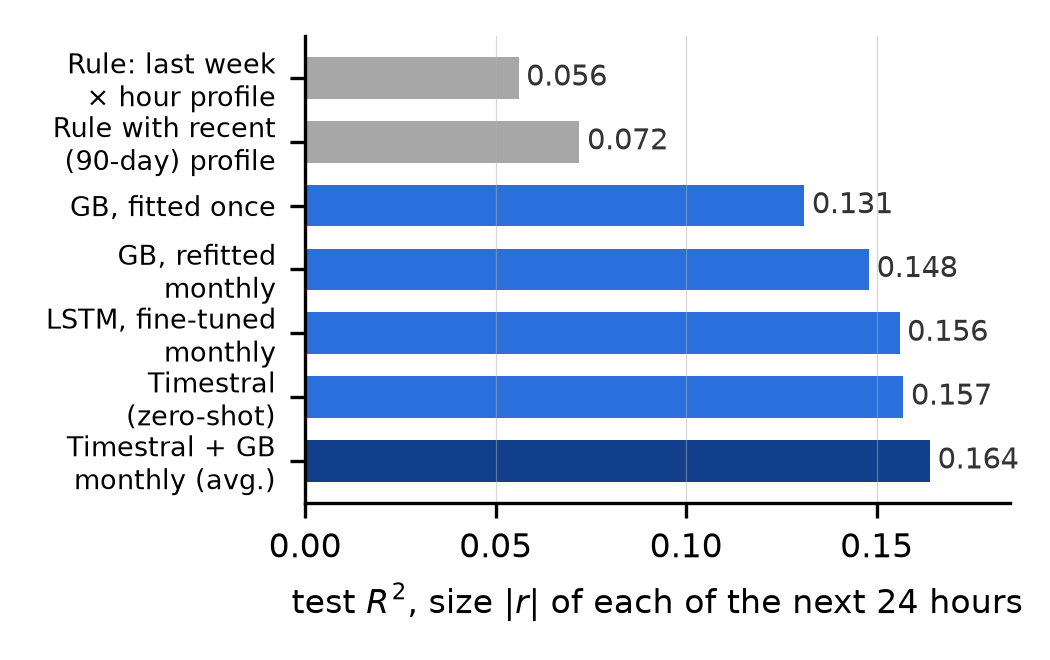
\includegraphics[width=0.9\columnwidth]{fig_size_r2.png}
  \caption{Test $R^2$ for the size of each of the next 24 hourly moves:
  simple rules (grey), single models (blue) and the chosen average of
  Timestral and monthly-refitted Gradient Boosting (dark blue).}
  \label{fig:size}
\end{figure}

\subsection{Prediction Ranges}
\label{sec:res_ranges}
The GB quantile ranges are 28\% narrower than a fixed range (0.92\%
vs.\ 1.28\%) and adapt to the market, but cover only 77.8\% of the test
hours: the test years differ from the training years. A correction
measured once on validation does not fix this (77.3\%), whereas rolling
conformal calibration, which keeps re-measuring the miss rate, does:
80.0\% coverage, 78\% in calm and 82\% in wild hours, at 0.98\% width,
while the fixed range over-covers calm hours (95\%) and under-covers wild
ones (80\%). Release hours are the weak spot: one factor for all hours
covers only 56\% of them; the Mondrian variant, chosen on validation,
lifts them to 82\% with ranges 2.08\% wide there. Timestral's quantiles
need no calibration: 80.3\% coverage at 1.00\% width, every one of its 21
quantile levels within 1.4 points of its nominal level, and the lowest
CRPS of the ranges tried (0.236 vs.\ 0.240 for a volatility-scaled
baseline); thanks to the release calendar it covers 70\% of the release
hours without any calibration, below Mondrian but 13.8 points $[+7.9,
+18.9]$ above a single rolling factor.

\subsection{Next-Day Targets and Economic Test}
\label{sec:res_daily}
At the daily scale, return and direction are not predictable (AUC
interval $[-0.023, +0.046]$ around 0.5), but volatility is: a top-3 tree
ensemble, chosen on walk-forward folds, explains 51\% of the next day's
log volatility, against 9.4\% for last week's average. A monthly refit of
GB raises its $\Rtwo$ from 0.503 to 0.517 ($+0.015$ $[+0.004, +0.025]$),
and averaging GB with an MLP adds $+0.011$ $[+0.001, +0.022]$ over GB.
On a small daily table of the next day's move size, plain Linear
Regression ($\Rtwo=0.514$) and SVR (0.519) beat Random Forest (0.464),
because tomorrow's volatility depends almost linearly on today's. A good
forecast is not a good strategy, though: volatility targeting with this
forecast (leverage capped at 2) reaches a Sharpe ratio of 0.27 after costs
against 0.50 for buy-and-hold (difference not significant, $[-0.57,
+0.11]$) and already lags before costs (0.41), because of its design: a
target level set on the more volatile training years, hence frequent
leverage, and daily turnover.

\subsection{Discussion}
\label{sec:discussion}
Because Bitcoin's behaviour drifts, models and calibrations that are
kept current beat models with more data or more inputs. A feature that carries information on its own (release
hours move 2--3 times more) does not help a model that already sees recent
volatility and the clock, or that has too few examples to use it; making
the release hours their own calibration group does. Model families
converge: GB, a carefully built LSTM and an untrained foundation model end
within 0.01 $\Rtwo$, and averaging two different families gives the best
result. Two caveats apply: there is a single test period of 2.25 years,
and Timestral was released after our test block without a list of its
training series; if Bitcoin 2023--2026 is among them, its scores are
optimistic.
